\section{Introduction}
A little longer version of the abstract.

Main goal: Argue for SC, and $x_Q$. Present $x_Q$ and justify decisions. Demonstrate the performance on `realistic simulations'.

within the scope of FAT* `topics of interest' we fall under the \emph{Transparency} branch. Specifically `Interpretability of ML models', and `Generation of explanations' (although probably more interpretability according to most people's definitions).

withing the scope of the FAT* tracks I believe that we align with:

\begin{enumerate}
    \item Statistics, Machine Learning, and Data Mining
    \item HCI, and Information Visualiation
    \item \ldots possibly something along the lines of empirical studies, as that is what we intend to do
\end{enumerate}

We can choose `archival' or `non-archival'. I think we probably want to do archival, since this is a promising `home' for our research anyway.

\subsection{Proposed outline:}

\begin{itemize}
    \item Motivation---why MDPs, why meta-analysis, why self-confidence?
    \item Related work---quickly review some related work in the area
    \item Approach---desiderata, Hellinger distance, etc
    \item Results/Discussion---Illustrative example, and theoretical example
    \item Conclusions/Future Work---restate purpose of SC, and particularly $x_Q$. Discuss continuing efforts to quantify effects with human-involved experiments. Further development of $x_H$, $x_I$, and $x_M$.
\end{itemize}

\subsection{Related Work}
    Discuss related work such as

    WHY DO WE USE MDPS? THEY ARE A GOOD PLACE TO START FROM, AND ARE CONNECTED TO MANY OTHER LEARNING APPROACHES (REINFORCEMENT, INVERSE REINFORCEMENT, \ldots)

    Reinforcement learning is finding a policy when transitions, and states are unknown. Basically learn policy and model simultaneously.

    inverse RL is learning a reward function by observing a policy.

\subsection{Factorized Machine Self-Confidence}
    Several definitions of self-confidence have been proposed in recent works. Much of this work is reviewed in \cite{Israelsen2017-ym}, where self-confidence is identified as an explicit assurances in a human-autonomy trust relationship. According to \cite{Sweet2016-tz} the four views on self-confidence are the \textit{anthropomorphic view}, the \textit{uncertainty view}, the \textit{experiential view}, and the \textit{stability view}. The anthropomorphic view defines self-confidence to be similar to how humans express self-confidence, while the experiential view expresses self-confidence based on past experience. The uncertainty view simply defines self-confidence to be the probability of success or failure, and the stability view defines self-confidence to be the sensitivity of the probability of success to uncertainty. All of these views seem to reflect different parts of a more general concept: understanding an autonomy's ability to do a specific task. This leads to the following definition of self-confidence.

    We define self-confidence to be: \textbf{An agent's perceived ability to achieve assigned goals (within a defined region of autonomous behavior) after accounting for (1) uncertainties in its knowledge of the world, (2) uncertainties of its own state, and (3) uncertainties about its reasoning process and execution abilities.}

    The formal definition of self-confidence we use is from \cite{Aitken2016-cv}, wherein five dimensions of self confidence are defined. They are:

        \begin{itemize}
            \item $x_I$ `Command Interpretation'
            \begin{itemize}
                \item are autonomy and user `on same page'?
            \end{itemize}
            \item $x_M$ `Model Validity'
            \begin{itemize}
                \item How well does autonomy's model reflect reality?
            \end{itemize}
            \item $x_Q$ `Solver Quality'
            \begin{itemize}
                \item how well can the solver use the model to generate policies/plans?
            \end{itemize}
            \item $x_P$ `Predicted Outcome Assessment'
            \begin{itemize}
                \item how `good' is expected distribution of results?
            \end{itemize}
            \item $x_H$ `Past Performance'
            \begin{itemize}
                \item how well has autonomy done in similar circumstances?
            \end{itemize}
            \item Assume that $SC = \mathsc{F}(X_{SC})\rightarrow [-1,1]$
        \end{itemize}

    Outcome assessment has been previously defined in \cite{Aitken2016-cv}, but has yet to been evaluated as an effective assurance as per the guidelines laid out in the work on assurances. Solver Quality is a metric that is, as yet, un-explored. The following are my targeted contributions for this work:

    \begin{itemize}
        \item Develop the $x_3$ `Solver Quality' (SQ) metric
        \item Develop a general approach for designing SC experiments
        \item Develop an experimental environment in which SC metrics can be evaluated with human participants
        \item Evaluate the `Predicted Outcome Assessment' metric developed by \cite{Aitken2016-cv}
    \end{itemize}

    \begin{figure*}[tbp]
        \centering
        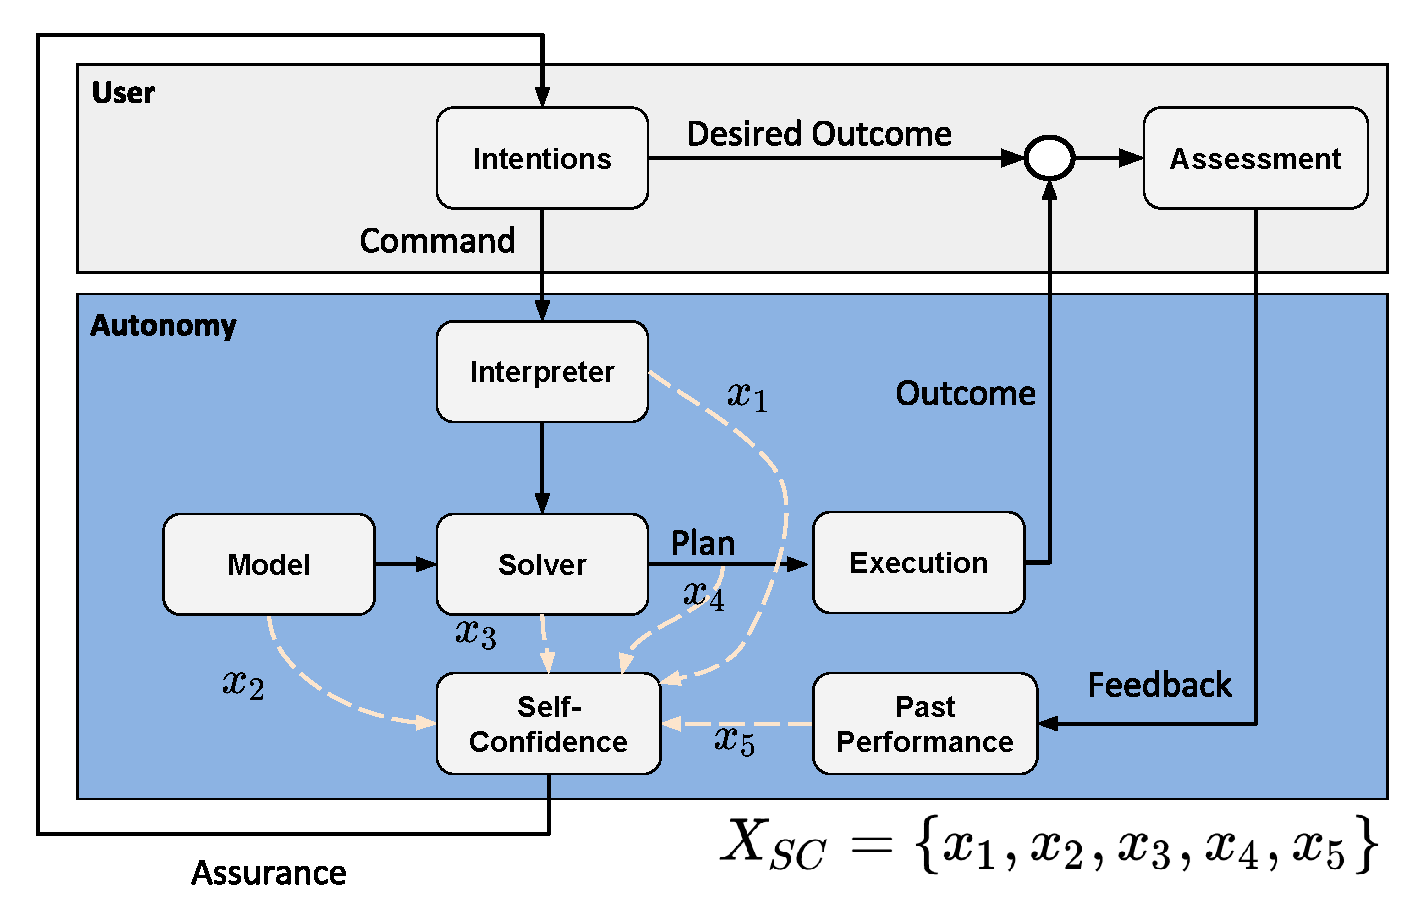
\includegraphics[width=0.65\linewidth]{Figures/SC_flowchart.pdf}
        \caption{Factorized Machine Self-Confidence}
        \label{fig:famsec}
    \end{figure*}

\subsection{Solver Quality}
    \begin{itemize}
        \item Desiderata
        \begin{itemize}
            \item appropriateness
            \item extend to unseen problems
            \item compare across solver classes
        \end{itemize}
    \end{itemize}
    The SQ metric is meant to address the question: ``How will a given solver $X$ perform on a given (possibly un-encountered) task''? Or, how well-suited is solver $X$ to investigating a certain task. Generally we want the following characteristics for SQ:

    \begin{itemize}
        \item Reflect the appropriateness of a solver for a given problem
        \item Useful for unseen problems (of similar type)
        \item Compare different classes of solvers
    \end{itemize}

    Solvers of all classes share two main properties. They operate on a specified problem, and solver parameters, in order to produce a policy $\pi$. Given the requirement to operate on different classes of solvers the SQ metric must operate on this high-level information. Namely, SQ should take, as inputs, the problem definition, and solver parameters, and produce some metric based on the resulting policy. This approach is inspired by \cite{Leyton-Brown2009-yr} who were able to use `Empirical Hardness Models' to predict the empirical runtime performance of an algorithm on a problem with given features. Figure~\ref{fig:SQ_flowchart} illustrates how this might work for SQ as an assurance. The idea is that SQ would be trained in a supervised manner before use, and then when presented with a task ascertain its performance.

    \begin{figure}[htbp]
        \centering
        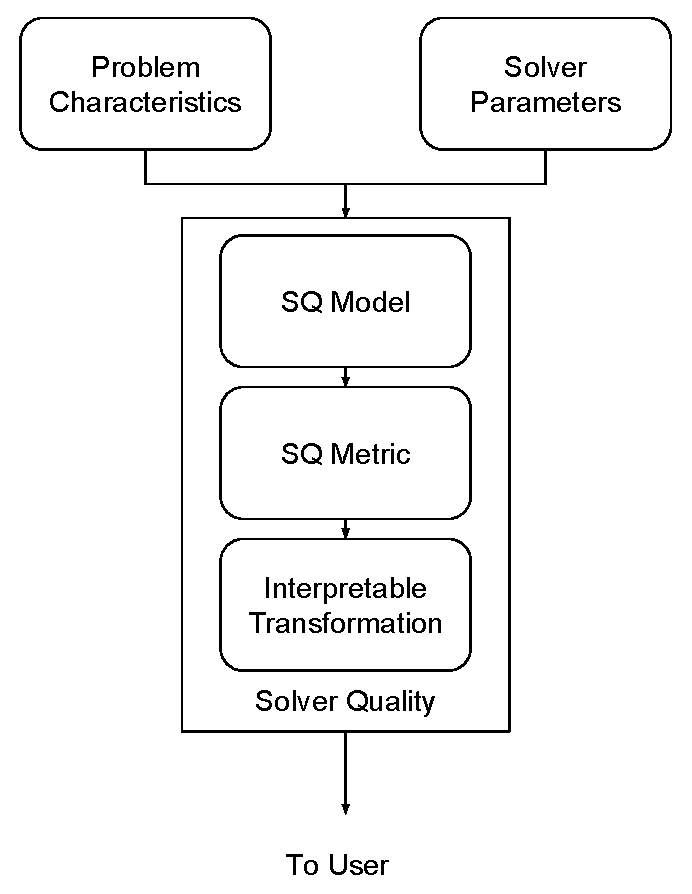
\includegraphics[width=0.3\textwidth]{Figures/SQ_EHM.pdf}
        \caption{Flowchart depicting how solver-quality metric could operate as an assurance.}
        \label{fig:SQ_flowchart}
    \end{figure}
    

    In order to evaluate the quality of some solver on a given problem $X$, we propose comparing the policy produced by that solver on $X$ to a `ground truth' policy $\pi^*$. This raises the question of how to compare policies. There are a few different approaches that present themselves:

    \begin{itemize}
        \item Compare utilities at each state
        \begin{itemize}
            \item Benefits: Evaluates whether states have similar utilities, quick to calculate
            \item Drawbacks: Does not apply to solvers that represent different amounts of the state-action space (i.e. exact vs. approximate solvers), or to solvers that may represent the state-action space differently (i.e. meta-solvers) 
        \end{itemize} 
        \item Compare `coverage' of the policy
        \begin{itemize}
            \item Benefits: Evaluates how thorough the policy is, quick to calculate
            \item Drawbacks: Similar limitations as above, not all policies will have the same coverage by design. Also a lot of coverage does not imply a `good' solution
        \end{itemize}
        \item Compare the reward distribution of given policies
        \begin{itemize}
            \item Benefits: Meets key desired properties (i.e. namely apply across different solver classes)
            \item Drawbacks: Expensive to calculate the reward distribution via many simulations
        \end{itemize}
    \end{itemize}
